\documentclass[article]{abntex2} 

\usepackage{graphicx}
\usepackage{hyperref}
\usepackage{blindtext}
\usepackage{float}
\usepackage{indentfirst}

\usepackage{listings}
\usepackage{color}


\definecolor{mauve}{rgb}{0.58,0,0.82}

\lstset{frame=tb,
  language=Java,
  aboveskip=3mm,
  belowskip=3mm,
  showstringspaces=false,
  columns=flexible,
  basicstyle={\small\ttfamily},
  numbers=none,
  numberstyle=\tiny\color{gray},
  keywordstyle=\color{blue},
  commentstyle=\color{dkgreen},
  stringstyle=\color{mauve},
  breaklines=true,
  breakatwhitespace=true,
  tabsize=3
}

\title{Trabalho Computacional\\ Transporte de Calor e Massa\\ Resolução da Equação do Calor utilizando o Método das Diferenças Finitas} 
\author{
 Emanuel Couto Brenag - 190057131
 \\Caso 7}      
\date{13 de Outubro, 2020}   
\tituloestrangeiro{}

\begin{document}            
\maketitle    
\thispagestyle{empty}
\clearpage
\pagestyle{plain}
\pagenumbering{arabic}
\newpage
\section{Introdução}
\subsection{A Equação do Calor}

 A equação geral da difusão de calor, também conhecida como equação do calor foi desenvolvida pela primeira vez por Fourier em 1822. Ela é estudada não só nos cursos de Transferência de Calor, mas também nos cursos de Física Matemática e Equações Diferenciais Parciais, sendo uma das principais equações da Termodinâmica Clássica (Pré-Mecânica Estatística). 
 
 A equação do calor, junto com suas variantes, também é importante em muitos campos da ciência e da matemática aplicada. Na teoria da probabilidade, a equação do calor está conectada com o estudo de passeios aleatórios e movimento browniano por meio da equação de Fokker-Planck. A infame equação de Black-Scholes da matemática financeira é uma pequena variante da equação do calor, e a equação de Schrödinger da mecânica quântica pode ser considerada uma equação do calor no tempo imaginário. Na análise de imagens, a equação do calor às vezes é usada para resolver a pixelização e identificar bordas. Seguindo a introdução de métodos de "viscosidade artificial" de Robert Richtmyer e John von Neumann, soluções de equações de calor têm sido úteis na formulação matemática de choques hidrodinâmicos. Soluções da equação do calor também têm recebido muita atenção na literatura de análise numérica, começando na década de 1950 com o trabalho de Jim Douglas, D.W. Peaceman e Henry Rachford Jr.
 
 A equação do calor é dada matematicamente por:
 $$ \rho C_{p} \frac{\partial T}{\partial t} = k \nabla^{2}T+H$$
 
 %colocar a eq
 
onde é $T$ é o campo de Temperatura,$\rho$ é a massa específica, $C_{p}$ é o calor específico a pressão constante, $k$ é a condutividade térmica do meio e $H$ representa a Geração interna de calor. Para esse caso específico, tomaremos a geração interna como diferente de zero. A partir dessa equação é possível descrever as variações de temperatura em um espaço em função do tempo, mas dependendo da malha a ser analisada, a complexidade aumenta e torna-se necessário o uso de métodos numéricos e computacionais para facilitar a resolução do problema. Para esse trabalho, utilizaremos o Método das Diferenças Finitas.


\subsection{O Método das Diferenças Finitas}
O Método das Diferenças finitas é a ferramenta numérica que torna mais prático a forma de resolver a equação do calor para problemas de dimensões maiores. A aproximação pelo médodo das diferenças finitas nos permite expressar a EDP do calor em conjuntos de pontos para assim determinar as temperaturas. Para isso, usamos aproximações e Séries de Taylor para transformar a equação diferencial em um sistema linear. Para o caso específico, temos um problema onde há geração interna de energia $H=10m^3/K$. 
Para utilizar o método, precisamos encontrar um jeito de desenvolver a equação bidimensional do calor de modo a discretizá-la e encontrar a equação de diferenças finitas em coordenadas cartesianas. 
$$k\frac{T_{m+1,n}^{p}+T_{m,n}^{p}+T_{m-1,n}^{p}}{\Delta x^2}+k\frac{T_{m,n+1}^{p}+T_{m,n}^{p}+T_{m,n-1}^{p}}{\Delta y^2}+H = \rho C_{p} \frac{T_{m,n}^{p+1}-T_{m,n}^{p}}{\Delta t}$$

Assumimos $\Delta = \Delta x = \Delta y $ e definimos o número de Fourier como: $$Fo=\frac{k\Delta t}{\rho C_{p} \Delta^2}$$
E a partir dessas definições e após efetuar algumas simplificações temos a discretização da temperatura para o método das diferenças finitas com geração interna de energia em cada ponto de uma malha dada por:
$$T_{m,n}^{p+1} = F_{o}(T_{m+1,n}^{p} + T_{m-1,n}^{p} + T_{m,n+1}^{p} + T_{m,n-1}^{p}) + (1-4F_{o})T_{m,n}^{p} + \frac{H\Delta }{k}^2 $$

Essa equação torna possível o desenvolvimento de um algoritmo computacional recursivo que descreva a difusão de temperatura no espaço e no tempo para diferentes geometrias.

\subsection{Objetivos}

\begin{itemize}
    \item Obter a solução numérica para 4 malhas com quantidades de nós distintas
    \item Plotar perfis de temperatura da malha mais refinada para 5 diferentes partes do domínio do cálculo
    %colocar aqui depois de ver com o tambs oq falta
    \item Computar o tempo computacional em função do número de nós
\end{itemize}

\begin{figure}[H]
    \begin{center}
       
        \includegraphics[scale=0.7]{Imagens/caso7.png} 
        \caption{Caso teste a ser simulado}
    \end{center}
\end{figure}
\section{Implementação}
\textbf{O código completo utilizado para gerar as simulações está comentado passo a passo e se encontra ao final desse relatório. Utilizarei essa seção do documento para explicar as partes mais importantes de sua implementação.}

Para a realização do projeto, optou-se pela linguagem Python, pela imensa possibilidade de bibliotecas prontas que poderia utilizar para a plotagem de gráficos e geração de animações das malhas. Além disso, os códigos rodam um pouco mais lentamente quando comparados com linguagens compiladas como C e C++, mas as facilitações das bibliotecas compensam esse tempo. MATLAB também era uma alternativa, porém a difícil acessibilidade e por ser mais pesado, se tornou inviável.

Para facilitar a geração das matrizes e a manipulação das mesmas, utilizou-se a biblioteca numpy. Para a plotagem de gráficos e animações se utilizou a extensa biblioteca matplotlib e por último, para o cálculo de custo operacional, a biblioteca time.

Além das bibliotecas, utilizaram-se  técnicas de desenvolvimento de software como a Programação Orientada a Objetos, com o intuito de facilitar a compreensão e manter o código mais sintetizado e econômico. 

\subsection{Ferramentas Computacionais}
Ao realizar o projeto, algumas ferramentas computacionais foram utilizadas de modo a tornar mais a realização do projeto. Para o desenvolvimento do código, utilizou-se a IDE Visual Studio Code, mas a ferramenta mais interessante para o desenvolvimento do projeto foi o Google Colab, que é uma plataforma Google que permite "emprestar" poder computacional dos servidores da Google, facilitando o desenvolvimento de simulações e tornando o procedimento mais rápido. O Colab foi um grande facilitador do projeto, visto que tornou o processo de geração do vídeo muito mais prático e rápido, além da ferramenta permitir compilar o código por partes, facilitando a maneira de encontrar erros no funcionamento do código.

\subsection{Criação da Malha}
O primeiro passo na realização das simulações foi estabelecer os valores das constantes utilizadas e também os valores das condições de contorno externas e internas (furo) do caso teste.
Para estabelecer as condições iniciais da malha optou-se por montar de uma maneira um pouco diferente. Foram utilizadas algumas funções da biblioteca math e algumas operações com matrizes para gerar a malha inicial. O código utilizado foi o seguinte:

\begin{figure}[H]
    \begin{center}
       
        \includegraphics[scale=0.7]{Imagens/boundary.png} 
        \caption{Trecho do código para estabelecer as condições iniciais}
    \end{center}
\end{figure}

\subsection{Iterações no Tempo}
A parte mais importante para conseguir estimar o modo como o calor flui são as iterações que ocorrem entre cada um dos nós da matriz utilizada. Cada uma dessas iterações representam um instante de tempo, e para cada um desses instantes foi gerado um novo elemento de um array de matrizes. Essa terceira dimensão dessas matrizes funcionava como o tempo. É importante mencionar que a cada iteração era necessário reafirmar as condições de contorno das bordas, visto que essas temperaturas deveriam se manter constante. O código utilizado para fazer essas iterações foi:

\begin{figure}[H]
    \begin{center}
       
        \includegraphics[scale=0.4]{Imagens/imagem_2020-10-16_164258.png} 
        \caption{Trecho do código responsável pelas iterações}
    \end{center}
\end{figure}



\subsection{Geração das Simulações}

Um dos maiores obstáculos na realização do código foi a geração das imagens. Definir as informações apresentadas nos gráficos, escolher um padrão de cores adequado e conseguir controlar a quantidade de frames e velocidade do vídeo foram coisas extremamente desafiadoras, tanto na implementação quanto para o computador operar. O código utilizado para gerar o vídeo e as imagens respectivamente foi:

\begin{figure}[H]
    \begin{center}
       
        \includegraphics[scale=0.5]{Imagens/imagem_2020-10-16_164802.png} 
        \caption{Trecho do código responsável pelas Simulações}
    \end{center}
\end{figure}



\subsection{Custo Computacional}



Para calcular o tempo operacional gasto pelo computador para gerar as malhas de diferentes números de nós, utilizei a função apresentada abaixo de modo que subtraí o tempo em que o código plota o gráfico do tempo em que começa a primeira das iterações e printo o número de segundos gastos para tal. A função recebe como argumento a Matriz, o número de Fourier e a geração interna e printa o tempo gasto.

\begin{figure}[H]
    \begin{center}
                \includegraphics[scale=0.7]{Imagens/tempo.png} 
        \caption{Função do tempo de operação}
    \end{center}
\end{figure}

O gráfico do tempo de execução do programa em função do número de nós é:



\begin{figure}[H]
    \begin{center}
        
        \includegraphics[scale=0.9]{Imagens/tempocomp.png} 
        \caption{Gráfico de Custo Operacional por Número de nós}
    \end{center}
\end{figure}

Ao desenvolver e testar o código ficou evidente o quão complexo se tornam os processos com o aumento do número de nós, porém é evidente que existe um acréscimo de caráter mais linear no tempo, visto que tudo que ocorre são operações com matrizes.

\section{Simulações}
As simulações computacionais em regime transiente foram feitas para um caso específico. Foram testados diversos materiais diferentes, porém o material que gerou as simulações mais estáveis possui as seguintes características: 

\begin{itemize}
    \item $\rho \approx 1800kg/m^3$ 
    \item $C_{p} \approx 1kJ/kgK$
    \item $k \approx 0,81W/m.K$
    \item $Fo= 0,25$ (para a malha mais refinada)
    \item $\Delta t= 0,5s$
\end{itemize}

O código é capaz de computar quaisquer valores de número de Fourier e Geração interna, mas escolhi a que achei que as simulações geradas eram mais estáveis e interessantes.
Para a escolha da malha mais refinada, foram observados diversos números de nós, porém para malhas maiores que 45x45 as diferenças no estado estacionário da simulação se tornavam cada vez mais imperceptíveis. A malha 90x90 é mais refinada que as anteriores e demorou um pouco mais para ser executada. Ela será utilizada para a análise dos perfis de temperatura posteriormente.

\subsection{Simulações para diferentes tamanhos de malha}

\begin{figure}[H]
    \begin{center}
       
        \includegraphics[scale=0.7]{certo1515.png} 
        \caption{Malha com 225 nós (15x15)}
    \end{center}
\end{figure}
\begin{figure}[H]
    \begin{center}
       
        \includegraphics[scale=0.7]{certo3030.png} 
        \caption{Malha com 900 nós (30x30)}
    \end{center}
\end{figure}
\begin{figure}[H]
    \begin{center}
       
        \includegraphics[scale=0.7]{certo4545.png} 
        \caption{Malha com 2025 nós (45x45)}
    \end{center}
\end{figure}
\begin{figure}[H]
    \begin{center}
       
        \includegraphics[scale=0.7]{5000-9090.png} 
        \caption{Malha com 8100 nós (90x90)}
    \end{center}
\end{figure}


\subsection{Perfis de Temperatura}
Os perfis de temperatura foram escolhidos com o propósito de verificar a temperatura da malha em regime permanente em algumas linhas da mesma. Cada um dos perfis mostra a propagação de calor para uma situação, sendo elas: proximidade das condições de contorno e o comportamento do campo de temperatura ao passar pelo furo adiabático da malha.

\begin{figure}[H]
    \begin{center}
       
        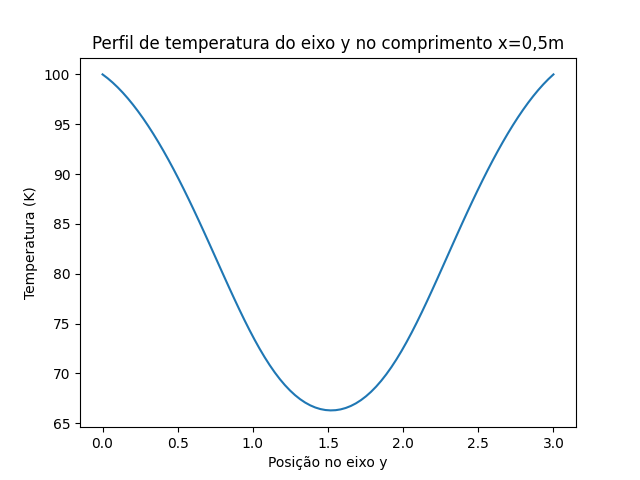
\includegraphics[scale=0.6]{perfilx=0,5.png} 
        \caption{Perfil de temperatura do eixo y em x = 0,5m}
    \end{center}
\end{figure}

       
Nesse primeiro perfil temos a temperatura de toda uma linha no eixo y onde x está em 0,5m. Essa linha cruza a malha de uma parede de 100K até outra parede de 100K, sem passar pelo buraco, porém pela influência das condições de contorno de temperatura da extremidade esquerda do buraco, podemos ver que ao cruzar o trecho onde temos o furo a temperatura cai, visto que lá as temperaturas são menores. Esse efeito também pode ser explicado pelo fato do trecho ser mais distante de ambas as bordas por estar no centro, e distante também da borda de 300K.

\begin{figure}[H]
    \begin{center}       
        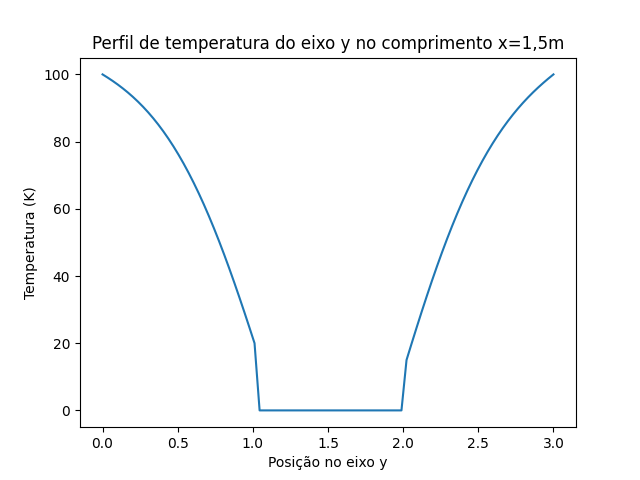
\includegraphics[scale=0.6]{perfilx=1,5.png} 
        \caption{Perfil de temperatura do eixo y em x = 1,5m}
    \end{center}
\end{figure}



Já nesse segundo perfil, que cruza o eixo y inteiro, tendo seu ponto fixo em x = 1,5m, podemos observar que esse ponto no eixo x passa exatamente pelo centro do furo da malha. Pode-se perceber uma descida estável na temperatura, provocada pelas condições de contorno que regem as temperaturas nas paredes do buraco. Além disso, percebe-se que em todo esse trecho adiabático, as temperaturas se encontram dentro do que é estabelecido pelo roteiro experimental (T=0K).

\begin{figure}[H]
    \begin{center}       
        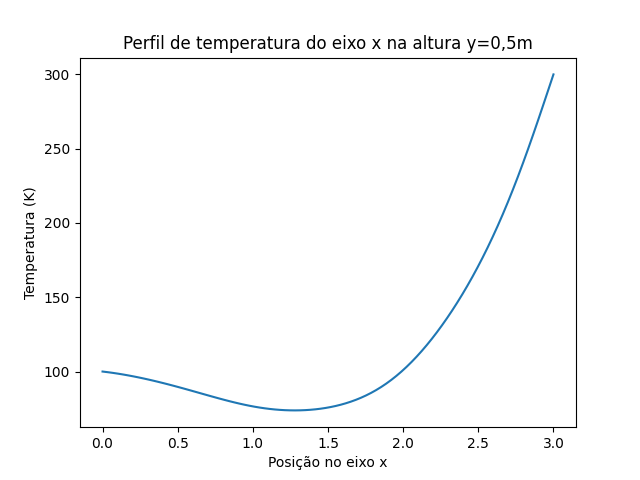
\includegraphics[scale=0.6]{perfily=0,5.png} 
        \caption{Perfil de temperatura do eixo x em y = 0,5m}
    \end{center}
\end{figure}

    
Para esse terceiro perfil, acontece o que é esperado: uma variação menos brusca da extremidade esquerda até o meio da malha, que tem temperaturas entre 10-20K, e depois a temperatura sobe de maneira muito rápida pela influência do fluxo de calor gerado pela borda que está aquecida a 300K.

\begin{figure}[H]
    \begin{center}
        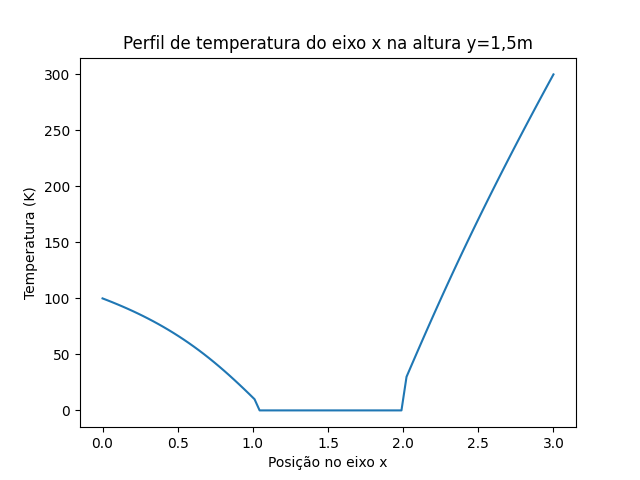
\includegraphics[scale=0.6]{perfily=1,5.png} 
        \caption{Perfil de temperatura do eixo x em y = 1,5m}
    \end{center}
\end{figure}


Assim como o terceiro perfil, esse quarto perfil tem uma variação menor da esquerda até o meio e uma subida extremamente brusca do meio até a borda direita, que é 3 vezes mais quente. O fato que diferencia essas duas bordas é que para percorrer esse caminho na altura y=1,5m, passa-se pelo buraco onde a temperatura é de 0K, sendo perceptível que a temperatura chega a 0 nesse momento e tem um degrau na saída do buraco, que pode ser explicado pela condição de contorno das bordas do mesmo.

    \begin{figure}[H]
        \begin{center}
        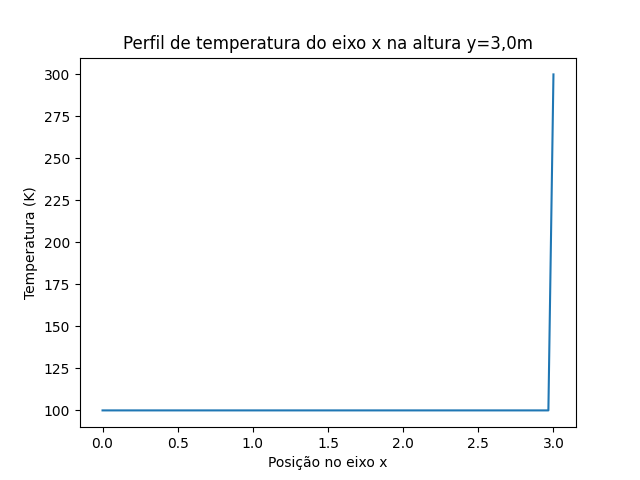
\includegraphics[scale=0.6]{perfily=3.png} 
        \caption{Perfil de temperatura do eixo x em y = 3m}
    \end{center}
\end{figure}

Esse quinto e último perfil de temperatura foi utilizado para verificar como o programa interpreta as condições de contorno em bordas de temperaturas muito diferentes. Cruzando o eixo x na altura máxima de y=3m, a borda tem temperatura constante de 100K, até chegar na extremidade onde a borda tem temperatura de 300K, que prevalece no nó, por isso ocorre essa subida linear, como um gráfico de uma função delta de Dirac.

\section{Comparações}
Foram plotadas simulações para a mesma malha, com mesmo Número de Fourier e quantidade de nós com o intuito de observar as mudanças que valores diferentes de geração interna de energia proporcionam. 

\begin{figure}[H]
    \begin{center}
       
        \includegraphics[scale=0.7]{Imagens/mtintGen.png} 
        \caption{Mapa de Calor com 10x mais geração interna}
    \end{center}
\end{figure}

Essa primeira figura representa uma malha com uma única alteração do valor de $H$, que variou de $10W/m^3$ para $100W/m^3$. Essa variação gera uma cor mais esverdeada na malha, que mostra que com essa grande geração interna, as temperaturas mais ao centro da distância entre a borda e o buraco são superiores às bordas de 100K. A temperatura volta a descer quando se aproxima do buraco, onde pode-se observar uma mudança extremamente brusca na temperatura, onde o tom de azul escurece bruscamente. 

\begin{figure}[H]
    \begin{center}
       
        \includegraphics[scale=0.7]{Imagens/semIntGen.png} 
        \caption{Mapa de Calor sem geração interna}
    \end{center}
\end{figure}

Ao comparar a malha sem geração interna de calor, podemos observar que as temperaturas se propagam de maneira muito parecida com a malha com a geração interna de $10W/m^3$, porém na malha com geração podemos observar que em cada um dos pontos as temperaturas são levemente superiores, com diferenças muito pequenas. Pode-se observar que próximo as bordas, os tons de azul permanecem claro por mais tempo ao se aproximar do meio da malha.


\section{Conclusão}
A partir do desenvolvimento computacional e de uma análise dos resultados obtidos pelas simulações, foi possível observar o modo como o calor flui em uma malha com diferentes temperaturas em cada uma de suas extremidades. Além disso, foi possível identificar o impacto causado por diferentes valores de geração interna. 
Pode-se concluir que o experimento foi um sucesso, visto que as comparações dos perfis e dos casos com diferentes gerações entregaram resultados que são tangíveis com a realidade. 

\section{Bibliografia}
As imagens utilizadas foram retiradas do roteiro do trabaalho computacional, localizado no site do Professor Rafael Gabler.
\newline

\begin{itemize}
    \item INCROPERA, Frank P. Fundamentos de Transferência de Calor e de Massa, LTC 8. Ed., 2019.
    \item VASCONCELOS, Marcelo Augusto. Uma Aplicação dos Métodos das Diferenças Finitas e Elementos Finitos a problemas térmicos. Orientador: Lineu José Pedroso. 2018. Monografia de Projeto Final em Estruturas, Universidade de Brasília, 2018.
\end{itemize}

\end{document}
